\documentclass{polytech-presentation}

\title{Développement d’un outil de traitement
d’images par filtrage bilatéral}
\author{Natacha \textsc{Marlio-Marette}}
\date{13/01/2015}

\begin{document}

\frame{\titlepage}	

	\begin{frame}<beamer>
    \frametitle{Plan}
    \tableofcontents
  \end{frame}

\section{Contexte}
	\subsection{Contexte}
		\begin{frame}
		\frametitle{Contexte}	
		\begin{block}{Filtre bilatéral}
		\begin{itemize}
			\item Utiliser pour lisser les détails en conservant les contours
			\item Utiliser pour manipuler les détails d'une image 
		\end{itemize}
		\end{block}			
		\end{frame}

	\subsection{Objectifs}
		\begin{frame}
		\frametitle{Objectifs}
			\begin{block}{Partie I}
				\begin{itemize}
					\item Impléméntation du filtre bilatéral
					\item Décomposition multi-échelle
					\item Manipulation des détails (2 niveaux)
				\end{itemize}
			\end{block}
		\pause
			\begin{block}{Partie II}
				\begin{itemize}
					\item Création de l'interface graphique
					\item Approximation rapide du filtre
				\end{itemize}
			\end{block}
		\end{frame}
		
		\begin{frame}
			\begin{block}{Partie III}
				\begin{itemize}
					\item Nouvelle méthode de décomposition
					\item Changement de la structure de l'image
					\item Travail sur les modèles 3D
				\end{itemize}
			\end{block}
		\end{frame}			
		
\section{Tâches}
		\begin{frame}
		\frametitle{Filtre bilatéral}	
		\begin{itemize}
			\item Implémentation du filtre
			\item Tests avec bruitage (bruit gaussien) et calcul du PSNR
			\item Echantillonage
			\item Trouver les paramètres $\sigma_s$ et $\sigma_r$ 
		\end{itemize}
		\end{frame}

		\begin{frame}
		\frametitle{Décomposition d'une image multi-échelle}
		\begin{itemize}
			\item Etude d'un article
			\item Décomposition de l'image par filtrage bilatéral itératif
			\item Tests 
		\end{itemize}
		\end{frame}
	
		\begin{frame}
			\frametitle{Manipulation des détails}
			\begin{itemize}
				\item Recomposition de l'image par combinaison linéaire
				\item Deux niveaux de détails : atténuation et rehaussement
			\end{itemize}
		\end{frame}
		
		\begin{frame}
			\frametitle{Création d'une interface graphique}
			\begin{itemize}
				\item Implémentation du MVC
				\item Création de l'IHM
				\item Ajout des fonctionnalités
			\end{itemize}
		\end{frame}
	
		\begin{frame}
			\frametitle{Approximation rapide du filtre}
			\begin{itemize}
				\item Etude d'un article
				\item Etude de l'implémentation MatLab
				\item Réalisation d'une nouvelle implémentation
				\item Comparaison avec CImg
			\end{itemize}
		\end{frame}
		
		\begin{frame}
			\frametitle{Modification de l'algorithme de décomposition}
			\begin{itemize}
				\item N'utilise plus le filtre bilatéral
				\item Méthode des moindres carrés
				\item Modification de la structure de l'image (structure de graphe)
			\end{itemize}
		\end{frame}
		
\section{Planning}
	\begin{frame}
		\frametitle{Planning}
		\begin{figure}
		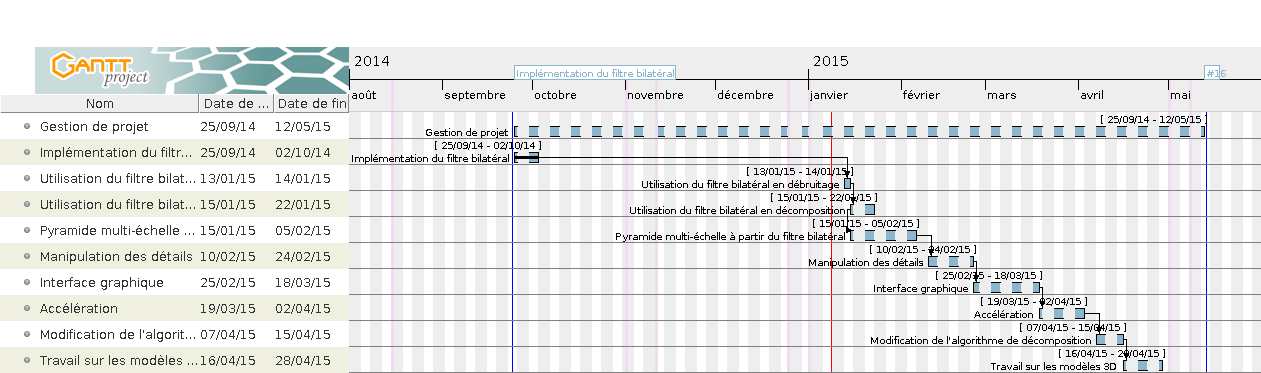
\includegraphics[width=320px]{../Gantt/Gantt.png} 
		%\caption{Planning}
		\end{figure}
		
	\end{frame}				
\end{document}
